\chapter{Introdução}
\label{intro}

A medição de sinais vitais é uma prática essencial para a avaliação das condições fisiológicas de um indivíduo e para garantir tratamentos adequados e evitar a deterioração de condições de saúde que podem ser prevenidas \cite{elliott2012vitalsigns}. Por esse motivo, no cenário clínico, especialmente no cuidado de pacientes de alto risco, há monitoramento contínuo com o uso de equipamentos médicos automatizados, a fim de possibilitar que mudanças significativas nos parâmetros fisiológicos possam ser prontamente identificadas e tratadas. A título de exemplo, a função cardíaca é tipicamente monitorada com o uso do eletrocardiograma (ECG), assim como a saturação de oxigênio é avaliada com o uso de oxímetros de pulso e a frequência respiratória é monitorada por pneumografia por impedância, que comumente utiliza os mesmos eletrodos que os equipamentos de ECG. 

No entanto, as restrições impostas pelo monitoramento contínuo por dispositivos com fios e contato direto com o corpo, principalmente durante períodos prolongados, podem gerar incômodo e são consideradas um dos fatores mais citados como agentes estressores para pacientes em Unidades de Terapia Intensiva (UTIs) \cite{ede2021ICUhumanfactors}. De fato, no contexto de Unidades de Terapia Intensiva Neonatal (UTINs), os dispositivos de medição requerem sensores adesivos que podem ocasionar lesões em recém-nascidos prematuros, os quais possuem a pele frágil, além de causar dor. Em contrapartida, soluções de medição de frequência cardíaca (FC), frequência respiratória (FR) e saturação de oxigênio  por câmera mostram acurácia clinicamente significativa e comparável aos métodos tradicionais nesse cenário \cite{villarroel2014neonatal}. 

Ademais, o monitoramento em UTIs apresenta desafios sobretudo durante o transporte de pacientes e devido ao mau contato dos sensores ou à má qualidade do sinal. Nesse caso, a monitorização por câmera se mostra uma alternativa capaz fornecer estimativas confiáveis das frequências cardíaca e respiratória e, principalmente, prever alterações no ritmo respiratório de forma condizente com o estado fisiológico em situações nas quais a aquisição por equipamentos de contato está ausente. Além disso, esse tipo de solução complementa essas medições e pode oferecer informações visuais sobre a morfologia do esforço respiratório e evidenciar assimetrias que contribuem para o diagnóstico de condições clínicas \cite{jorge2022postOpICU}.

A partir disso, diante dos desafios impostos pela aquisição de sinais vitais por meio de equipamentos médicos de contato, a medição de parâmetros fisiológicos por câmera apresenta-se como uma estratégia confiável e possui vantagens de custo e facilidade de aplicação comparado a outras estratégias de monitorização remota, como as baseadas em indução magnética, efeito Doppler ou imageamento térmico \cite{khanam2019clinicalnonclinicalReview}. Nesse sentido, as soluções de medição por câmera baseiam-se, principalmente, em métodos de fotopletismografia remota (rPPG), os quais possuem o objetivo de detectar as variações cíclicas do sistema cardiovascular que podem ser extraídas a partir das mudanças sutis de intensidade dos elementos de cor de uma área do corpo ao longo do tempo. Assim, a luz que é re-emitida após passar pelos tecidos da pele é captada por dispositivos de aquisição de imagens, sendo que as propriedades óticas da superfície do corpo são influenciadas sobretudo pela hemoglobina e pela melanina da região analisada. Em função das características descritas, as principais aplicações utilizam não só câmeras RGB convencionais, mas também câmeras sensíveis ao infravermelho ou ao infravermelho próximo \cite{selvaraju2022continuous}.

Dessa forma, a compreensão detalhada da fotopletismografia remota requer, inicialmente, a definição dos princípios básicos da fotopletismografia (PPG). A PPG é uma técnica ótica de medição que pode ser utilizada para detectar variações no volume sanguíneo no leito microvascular dos tecidos. Desse modo, o sinal característico dessa técnica possui uma componente pulsátil chamada de componente AC com frequência fundamental próxima a 1 Hz e que depende do batimento cardíaco, conforme ilustra a Figura \ref{fig:ppgWave}. Analogamente, há uma componente DC que varia lentamente de acordo com a respiração, com a atividade vasomotora e com ondas vasoconstritoras, além de ondas Traube-Hering-Mayer (THM) relativas a oscilações da pressão arterial. Esse sinal pode ser percebido devido às características óticas da pele, sendo que os fatores primordiais que afetam a quantidade de luz recebida por um fotodetector de um tecido iluminado são o volume sanguíneo, a movimentação das paredes dos vasos e a orientação das células vermelhas. Há, ainda a influência do comprimento de onda da fonte na interação entre a pele e a luz, de modo que a medição convencional desse sinal, tipicamente realizada por oxímetros de pulso, utiliza feixes na faixa do vermelho e do infravermelho para detecção da saturação periférica de oxigênio baseada nas propriedades óticas de absorção da oxihemoglobina e da desoxihemoglobina nessas regiões do espectro eletromagnético \cite{allen2007photoplethysmography}.

\begin{figure}[H]
    \centering
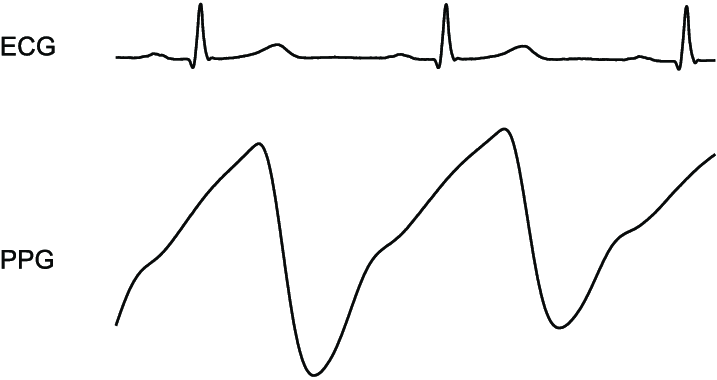
\includegraphics[width=0.6\linewidth]{imagens/PPGwaveAllen2007.png}
    \caption{Componente pulsátil do sinal de PPG e o ECG correspondente} 
    Fonte: \citeonline{allen2007photoplethysmography}
    \label{fig:ppgWave}
\end{figure}

Diante do exposto, a literatura mostra que é possível obter um sinal de PPG de forma remota com o uso de câmeras convencionais e utilizando a luz ambiente como principal fonte de iluminação, por meio da análise das variações dos canais de cor de regiões de interesse específicas \cite{verkruysse2008remote}. Além disso, a fim de definir princípios bem estabelecidos para a extração de sinais de rPPG, os principais métodos consideram a modelagem da interação entre a luz e a pele com base na lei de Beer-Lambert, a qual descreve como a absorção da luz por uma substância depende de sua concentração e do caminho percorrido pelo feixe, ou no modelo dicromático de reflexão de Shafer, o qual define que a luz refletida por um material dielétrico não homogêneo pode ser dividida em uma componente de reflexão difusa e uma componente de reflexão especular \cite{chen2018deepphys}.

Nesse contexto, a extração do sinal de rPPG pode ser realizada tanto com o uso exclusivo de luz ambiente quanto por meio de fontes de iluminação controladas, com um ou mais dispositivos de aquisição de imagens para a captura de dados de vídeo \cite{mcduff2015survey}. A metodologia usual envolve a detecção e o rastreamento de uma região de interesse (ROI), a partir da qual é obtido o sinal bruto por meio da análise dos canais de cor dos pixeis de cada frame. Posteriormente, esse sinal é filtrado e processado a fim de reconstruir a onda de pulso de volume sanguíneo (BVP) característica da fotopletismografia, cujas propriedades podem ser utilizadas para a estimação de parâmetros fisiológicos \cite{rouast2018review}, conforme esquematiza a Figura \ref{fig:rppgschematic}.

\begin{figure}[H]
    \centering
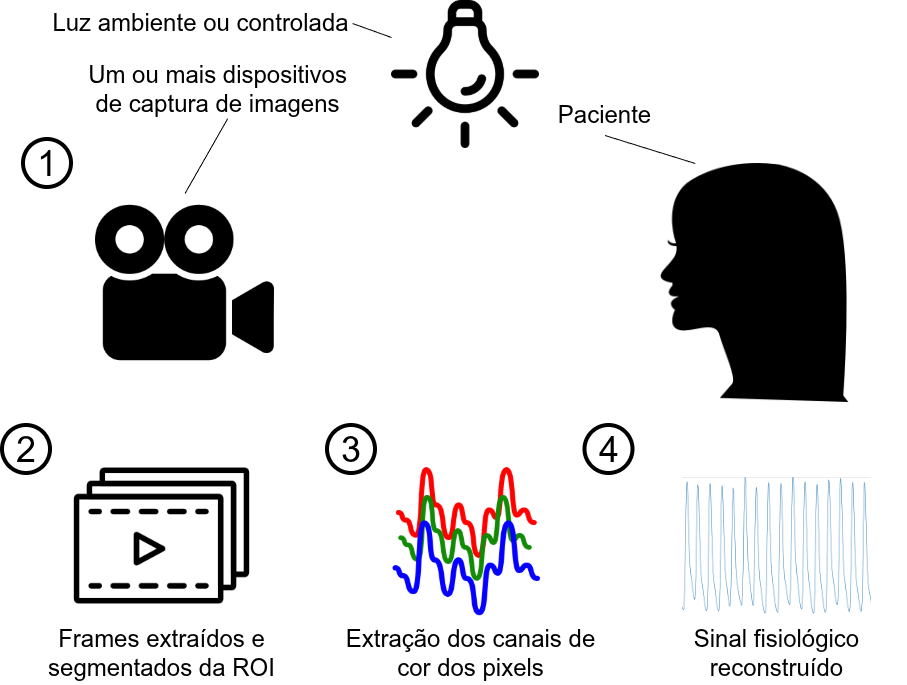
\includegraphics[width=0.6\linewidth]{imagens/rPPGschematic.png}
    \caption{Esquemático da extração de sinais por fotopletismografia remota} 
    Fonte: Adaptado de \citeonline{mcduff2015survey}
    \label{fig:rppgschematic}
\end{figure}

Por conseguinte, as principais implementações utilizam métodos não supervisionados, bem como métodos baseados em aprendizado profundo (\textit{deep learning}, DL). Os métodos não supervisionados extraem os sinais fisiológicos por estratégias de análise de cor ou de movimento das imagens de entrada. Sistemas baseados em DL, por sua vez, utilizam tanto modelos fim a fim, os quais são treinados para extraírem o sinal de rPPG ou diretamente parâmetros fisiológicos a partir de dados de vídeo como entrada, quanto sistemas híbridos, os quais combinam métodos algorítmicos com modelos de DL que extraem características específicas em uma ou mais partes do processo de estimação de parâmetros. Desse modo, pode-se extrair dados de perfusão sanguínea periférica, frequência respiratória, saturação de oxigênio, frequência cardíaca e de pulso, variabilidade das frequências cardíaca e de pulso e pressão arterial por meio das diferentes abordagens \cite{chen2024deep}.
 
 Em vista disso, a extração do sinal de rPPG possui crescente potencial de aplicabilidade, por exemplo, no monitoramento dos parâmetros fisiológicos de pacientes em sessões de tratamento de hemodiálise. Nesse cenário, algoritmos de imageamento fotopletismográfico podem estimar valores de frequência cardíaca com boa concordância em relação aos adquiridos por equipamentos médicos de referência \cite{villarroel2017non, villarroel2020non}. Adicionalmente, nesse mesmo contexto clínico, os sinais de frequência respiratória adquiridos por esses métodos podem ser considerados mais estáveis que os obtidos com a utilização de cintas torácicas \cite{tarassenko2014non}. 
 
 Outro tipo de aplicação envolve a detecção de fibrilação atrial com base no sinal de fotopletismografia obtido remotamente. Para isso, é possível analisar índices estatísticos de variabilidade da frequência cardíaca baseados no pulso extraído dos dados de vídeo dos indivíduos analisados \cite{couderc2015detection}. Ademais, pode-se utilizar modelos de aprendizado profundo para classificar os sinais de rPPG de pacientes, de modo a indicar se possuem essa condição, se possuem ritmo sinusal normal ou outros tipos de alterações no ritmo cardíaco \cite{sun2022contactless}.

Observa-se, ainda, que a medição de sinais vitais de forma remota possui relevância no contexto de missões de busca e resgate para triagem de vítimas, sendo que há implementações que envolvem a aquisição de vídeos por câmeras embarcadas em veículos aéreos não tripulados. A partir dessas imagens, é possível extrair sinais de frequência cardíaca e respiratória com boa concordância em relação a dispositivos de referência como transdutores piezoelétricos de cinta respiratória e oxímetros de pulso. Nesse caso, a utilização de algoritmos de redução de ruídos é essencial para minimizar a influência de variações de iluminação e da movimentação tanto da câmera quanto dos indivíduos monitorados \cite{al2017remote}.

De modo complementar, a fotopletismografia remota possui potencial de aplicação para disparo cardíaco em procedimentos de ressonância magnética. A obtenção da onda de rPPG pode ser utilizada para iniciar a captura de imagens em momentos específicos do ciclo cardíaco. Esse tipo de abordagem, sobretudo na aquisição realizada por equipamentos de campo ultra-alto, evita o contato físico e possui menor interferência de artefatos em relação à oximetria de pulso e ao eletrocardiograma, que são os principais métodos de contato utilizados nesse contexto \cite{spicher2016initial}. 

O monitoramento remoto de parâmetros fisiológicos apresenta, adicionalmente, vantagens em relação a abordagens convencionais sobretudo no que se refere à realização de exercícios físicos, em que a medição por contato é dificultada \cite{napolean2022heart}. Durante a prática esportiva, as frequências cardíaca e respiratória são importantes para o cálculo do índice de intensidade de atividade física o qual, por sua vez, possibilita uma análise do esforço realizado. Assim, é possível evitar lesões por meio da identificação de condições de fadiga extrema a partir desse índice, que pode ser obtido com base nos sinais extraídos por câmera \cite{wu2023motion}. 

Com base nas discussões apresentadas, é observável a importância da aquisição de sinais vitais para acompanhamento do status fisiológico de indivíduos em diversos contextos. Desse modo, diante das limitações impostas pela medição por equipamentos convencionais, implementações de monitorização sem contato, sobretudo a fotopletismografia remota, apresentam significativo potencial a ser explorado principalmente no ambiente clínico. Por isso, esse projeto visa aplicar os principais algoritmos e estratégias de estimativa de parâmetros fisiológicos por rPPG em vídeos adquiridos de pacientes admitidos em uma Unidade de Terapia Intensiva, a fim analisar o desempenho desse tipo de solução no cenário de cuidado crítico.
    
    \section{Objetivos}

    Este trabalho possui dois objetivos principais. Primeiramente, o desenvolvimento de uma base de dados para rPPG de pacientes admitidos na Unidade de Terapia Intensiva do Hospital Universitário (HU) da Universidade de São Paulo (USP). Para isso, é realizada a coleta de vídeos e, simultaneamente, são adquiridos os sinais correspondentes dos monitores multiparamétricos da instalação de saúde como valores de referência. A partir disso, objetiva-se, adicionalmente, reproduzir os principais algoritmos de fotopletismografia remota para estimativa de parâmetros fisiológicos e aplicá-los aos dados coletados, a fim analisar o desempenho dessas implementações em um ambiente realista de cuidado crítico. Assim, discerne-se esses objetivos gerais em objetivos específicos:
    \begin{itemize}
        \item Coletar dados de vídeo e medições de referência correspondentes de pacientes em uma Unidade de Terapia Intensiva
        \item Reproduzir os principais algoritmos não supervisionados de fotopletismografia remota
        \item Reproduzir as implementações de rPPG baseadas em aprendizado profundo de maior relevância na literatura e que possuem modelos e parâmetros de acesso aberto
        \item Avaliar os métodos reproduzidos nos dados coletados com base em métricas bem definidas
        \item Comparar o desempenho obtido nos dados coletados com o desempenho em bases de dados disponíveis na literatura
        
    \end{itemize}
    
 \section{Justificativa}

      É visível o potencial e a ampla gama de aplicações de soluções de monitoramento sem contato baseadas em fotopletismografia remota. No entanto, as implementações nesse contexto possuem como limitação a escassez de estudos em condições realistas como em hospitais e clínicas, sendo que a literatura é baseada predominantemente em ambientes controlados e análises com pacientes saudáveis \cite{bautista2023clinical, harford2019availability}. Em vista disso, este projeto visa contribuir com uma investigação sobre a aplicação da rPPG em um cenário real de forma inédita em uma instituição de saúde pública brasileira a qual faz parte do Sistema Único de Saúde, envolvendo pacientes críticos de forma a analisar o desempenho dos métodos desenvolvidos nesses casos, bem como disponibilizar a base de dados obtida para desenvolvimentos futuros.
	